\documentclass[a4paper,12pt]{article}

% Font
\usepackage[T1]{fontenc}
\usepackage{gentium}

% Math packages
\usepackage{amsmath}
\usepackage{amsfonts}
\usepackage{amssymb}
\usepackage{amsthm}
\usepackage{bm}

% Define symbol shortcuts
\newcommand{\cc}{\mathcal{C}}
\newcommand{\dd}{\mathcal{D}}
\newcommand{\hh}{\mathcal{H}}
\newcommand{\xx}{{\bm x}}
\newcommand{\yy}{{\bm y}}

% Math environment
\newtheorem*{thm}{Theorem}

% Better list management:
% - vertical spacing in lists
% - items in lists start with dash not bullet point.
\usepackage{enumitem}
\setlist{label=\textemdash,
  itemsep=0pt, topsep=3pt, partopsep=0pt} 

% Include graphics
\usepackage{graphicx}
\usepackage{subcaption}

% Page format 
\usepackage[top=2cm,left=2cm,right=2cm,bottom=2cm]{geometry}

\begin{document}
%%% HEADER
% \raisebox{0.6in}[0in]{\makebox[\textwidth][r]{\it Unproofed version }}
% \vspace{-0.7in}

\begin{center}
\bf\large MA2823: Foundations of Machine Learning \\
Chapter 2: Supervised Learning
\end{center}

\noindent
Lecturer: Chlo\'e-Agathe Azencott   
\hfill
Scribe: Chlo\'e-Agathe Azencott

\noindent
\rule{\textwidth}{1pt}

\medskip

%%% NOTES START HERE
In this chapter we will see:
\begin{itemize}
\item how to formulate a supervised machine learning problem;
\item some basic elements of learning theory;
\item how to define and use the notion of model complexity.
\end{itemize}

\section{Supervised classification}
The goal of {\em supervised classification} is to learn a class of objects from examples. Let us define a $p$-dimensional representation of the objects of interest. 

\paragraph{Definitions and notations.} Let us consider that we are given $n$ {\em training examples}, or {\em training (data) points}, or {\em observations}, or {\em training samples}. These $n$ points form the {\em training set}, and are represented by $n$ $p$-dimensional vectors $\{\xx^1, \dots, \xx^n\}$: $\xx^i \in \mathbb{R}^p, i \in \{1, \dots, n\}$. The $p$ dimensions chosen to represent the data are called {\em features}, {\em descriptors}, {\em variables} or {\em attributes}. Finally, the {\em training set} also contains the {\em labels}, {\em or targets}, or {\em outcomes} $\{y^1, \dots, y^n\}$: $y^i \in \{0, 1\}$. For any $i \in \{1, \dots, n\}$,  $y^i = 1$ if and only if $\xx^i$ represents an object that belongs to $\cc$. In that case, $\xx^i$ is said to be a {\em positive example}. If it does not belong to $\cc$, $y^i=0$ and $\xx^i$ is called a {\em negative example}. \\

The training set is denoted by $\dd = \{ (\xx^1, y^1), (\xx^2, y^2), \dots, (\xx^n, y^n) \}$.
The goal of {\em supervised classification} is to use $\dd$ to define a function $f: \mathbb{R}^p \rightarrow \{0, 1\}$ that returns $1$ if and only if it is given as input an object that belongs to $\cc$. 
We will use $c: \mathbb{R}^p \rightarrow \{0, 1\}$ to denote the true function that accurately labels data points and that we want to approximate.

\paragraph{Empirical error.} On the training set $\dd$, the {\em empirical error} of $f$ is given by 
\[
E(f|\dd) = \frac{1}{n}\sum_{i=1}^n 1_{f(\xx^i) \neq y^i}.
\]
It counts the number of mistakes made by the classifier.

\section{Version space} 
Our beliefs about the class $\cc$ allows us to define the {\em hypothesis space $\hh$} from which we believe $\cc$ to be drawn. We will be looking for a prediction function (or {\em discriminant}) $f \in \hh$.\\

One of the central questions in machine learning is to define the hypothesis space $\hh$. Another one is to formulate ways to choose $f \in \hh$. One of our main concerns will be {\em generalization}: we want $f$ to work well on data other than the training data, i.e. data that we have not observed yet. With this in mind, we can define the {\em most speficic hypothesis} as the hypothesis $S \in \hh$ that is most tight to the positive training examples. We can also define the {\em most generic hypothesis} as the hypothesis $G \in \hh$ that is most tight to the negative training examples.\\

Ideally, with enough training samples, the most specific and the most generic hypotheses coincide.
This can be illustrated with a card classification example. We are going through a deck of cards, and are being told for each card whether it is a ``good card'' (positive class) or a ``bad card''. Before we start, the most specific hypothesis is that there is no good card. The most generic hypothesis is that all cards are good cards. After each card we see, we can update the hypotheses, until they converge.\\

However, it is generally the case that we do not have enough training points to make the most specific and the most generic hypotheses match. In that setting, all hypotheses that are between $S$ and $G$ are said to be {\em consistent} with the training data $\dd$. This means that these hypotheses do not make any mistake on the training set. Their empirical error on $\dd$ is $0$. The set of consistent hypotheses is called the {\em version space}. This concept was defined by Tom Mitchell in the early 1980s.\\

One possible strategy is to choose $f$ half-way between $S$ and $G$. This strategy maximizes the {\em margin}, that is to say the distance between the decision boundary and the nearest point from the training set.



\paragraph{Example.} Let us look at objects that are cars and are represented by a $2$-dimensional representation: $x_1$ is the price of car $\xx$ and $x_2$ is its engine power. Let $\cc$ be the class of ``family cars''. 

Our goal is to define a function $f: \mathbb{R}^2 \rightarrow \{0, 1\}$ that only returns $0$ if $(x_1, x_2)$ represents a family car. This example is illustrated on Fig.~\ref{fig:car_data}. 

In this case, what we believe about family cars is that they are of medium-range prices and medium-range engine power. Formally, this means we believe $\cc$ to be a rectangle aligned with the axes, defined by $p_1 \leq x_1 \leq p_2$ and $e_1 \leq x_2 \leq e_2$. Our hypothesis space is the set of axis-aligned rectangles.

\begin{figure}[h]
  \centering
  \begin{subfigure}[c]{0.45\textwidth}
    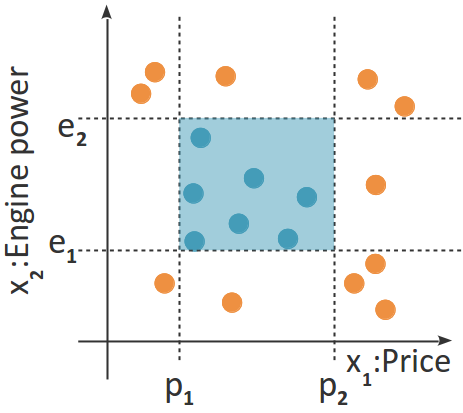
\includegraphics[width=0.7\textwidth]{figures/car_data}
  \end{subfigure} \hfill
  \begin{subfigure}[c]{0.45\textwidth}
    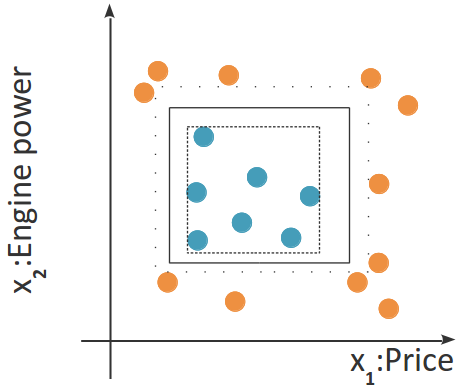
\includegraphics[width=0.7\textwidth]{figures/car_data_2}
  \end{subfigure}
\caption{Left: Training data for the class "family cars". Blue points are family cars, orange points are not. We believe the discriminant to be an axis-aligned rectangle and $\cc$ to be defined by $p_1 \leq x_1 \leq p_2$ and $e_1 \leq x_2 \leq e_2$. Right: the most specific hypothesis (dashed), the most generic hypothesis (dotted), and the margin-maximizing hypothesis (continuous).}
  \label{fig:car_data}
\end{figure}


\section{Model complexity}
\subsection{Overfitting}
In real-world applications, there are multiple sources of noise in the training data:
\begin{itemize}
\item {\em measurement noise}, i.e. imprecision in recording the features that describe the data;
\item {\em teacher noise}, i.e. errors in data labeling;
\item missing features, i.e. hidden (or {\em latent}) factors that would be necessary to be able to really make the classification.
\end{itemize}
This means that it might not be possible to make no error on the training set.

In addition, aiming at all cost to fit the training data might result in {\em overfitting}: the model is too complex and is not likely to generalize well. This happens when $\hh$ is more complex than $\cc$.

On the contrary, {\em underfitting} takes place when the hypothesis space is too simple, and no function from $\hh$ can fit the training data well enough to have a good chance to generalize. 

Both behaviors are illustrated on Fig.~\ref{fig:model_complexity}.
\begin{figure}[h]
  \centering
  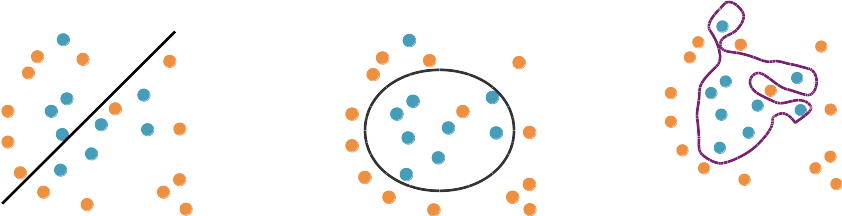
\includegraphics[width=0.6\textwidth]{figures/model_complexity}
  \caption{Models of increasing complexity. The simple straight line on the left might underfit. The complex line on the right is likely to overfit. }
  \label{fig:model_complexity}
\end{figure}

We tend to favor using simpler models when possible (i.e. when they are not likely to underfit): 
\begin{itemize}
\item they are easier to use (lower computational complexity);
\item they are easier to train (lower space complexity);
\item they are easier to interpret;
\item they tend to generalize better;
\item Occam's razor suggests that simple explanations are more plausible.
\end{itemize}


\subsection{Bias-Variance tradeoff}
In statistics, {\em bias} is the difference between the expected value of an estimator and the true value being estimated:
\[
\mbox{Bias}(\hat y) =  \mathbb{E}\left( \hat y - y \right).
\] 
A simpler model has a higher bias (it makes mistakes on the training data): high bias can cause underfitting.

The {\em variance} of an estimator is the deviation of the estimates from the expected values:
\[
\mbox{Variance}(\hat y) = \mathbb{E}\left( \hat y - \mathbb{E}(\hat y) \right).
\]
A more complex model has higher variance. High variance can cause overfitting.\\

In other words, increasing model complexity towards overfitting decreases the bias and increases the variance. Conversely, decreasing model complexity towards underfitting increases the bias and decreases the variance. This behavior is illustrated on Fig.~\ref{fig:bias_variance}. We must be wary of wanting to minimize bias at all costs, as it might result in a worse model.\\

The mean squared error of the prediction, $\mbox{MSE} =  \mathbb{E} \left( \hat y - y)^2 \right)$, can be rewritten as $\mbox{MSE} = \mbox{Var}(\hat y) + \mbox{Bias}^2(\hat y)$. This is refered to as the {\em bias-variance decomposition}, and illustrate that there is a tradeoff between bias and variance.

\begin{figure}[h]
  \centering
  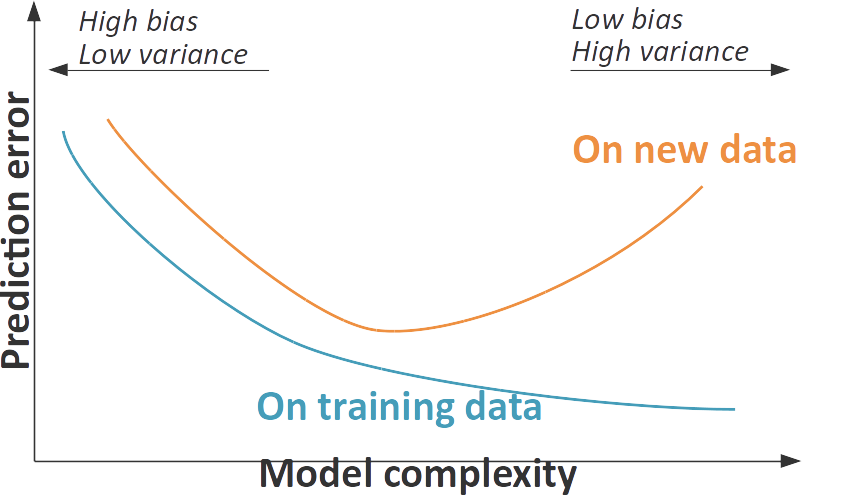
\includegraphics[width=0.5\textwidth]{figures/bias_variance}
  \caption{Bias-variance trade-off.}
  \label{fig:bias_variance}
\end{figure}

\section{Complexity of the hypothesis space: Vapnik-Chervonenkis dimension}

Let us consider $N$ points. There are $2^N$ ways in which these points can be labeled positive and negative. The hypothesis space $\hh$ is said to {\em shatter} $N$ if, for any of these $2^N$ labelings, there exists a hypothesis $h \in \hh$ that is consistent. The {\em Vapnik-Chervonenkis dimension} (or {\em VC-dimension}) of $\hh$ is the maximum number of points that can be shattered by $N$. The VC-dimension was defined by Vapnik and Chervonenkis in 1970.

\paragraph{Example: VC-dimension of a line (in $\mathbb{R}^2)$.} There exist configurations of $3$ points such that, whatever their labels, one can find a line that separates the positive point(s) from the negative point(s). However, there is no configuration of $4$ points such that, whatever their labels, one can find a line that separates the positive point(s) from the negative point(s). The VC dimension of a line is $3$.

\paragraph{Example: VC-dimension of an axis-aligned rectangle (in $\mathbb{R}^2)$.} There exist configurations of $4$ points (for example on the vertices of a parallelogram that is not aligned with the angles) such that, whatever their labels, one can find a rectangle that separates the positive point(s) from the negative point(s). However, there is no configuration of $5$ points such that, whatever their labels, one can find a rectangle that separates the positive point(s) from the negative point(s). Hence the VC dimension of a rectangle is $4$. 

This suggests that, using an axis-aligned rectangle, we can only guarantee learning datasets with $4$ data points: if there are more, the rectangle might not be consistent with the data. 

However, the VC-dimension is independent of the probability distribution of the data we are interested in. The world changes smoothly, and, especially for well-designed representations, nearby instances tend to have the same label. Hence we can still learn specific classes with an hypothesis space of low VC-dimension.

\section{Probably Approximately Correct learning}

PAC-learning is a theoretical framework for the mathematical analysis of machine learning that was proposed by Leslie Vaillant in 1984. 

PAC-learnability rests on the two following concepts:
\begin{itemize}
\item $f$ must be {\em approximately correct}, that is to say, the probability that $f$ makes a mistake must be bounded by $\epsilon > 0$: 
$P_{\dd}(f(x) \neq c(x)) \leq \epsilon$.
\item $f$ must be {\em probably correct}, that is to say, $f$ is correct most of the time, i.e. with probability at least $1-\delta$, where $\delta \leq \frac{1}{2}$. 
\end{itemize}
A probably approximately correct hypothesis $f$ verifies
\[
P_{\dd}\left(
P_{\dd}(f(\xx) \neq c(\xx))
\leq \epsilon \right) \geq (1 - \delta).
\]

$P_\dd$ refers to the probability over which training examples you happen to get when building $\dd$.



A hypothesis class $\hh$ is said to be {\em PAC-learnable} if, for any class $\hh \subset \cc$, for any training dataset $\dd$, there exists an algorithm that produces a probably approximately correct hypothesis in polynomial time in $1/\epsilon$ and $1/\delta$.

In that case, its {\em sample complexity} is the number $n$ of training examples that it needs in order to learn a probably approximately correct hypothesis. 

This means that, given $\epsilon$, $\delta$, and a class $\cc$ from which the training data $\dd$ is drawn, we want to find $n$ such that 

\paragraph{Example: Learning axis-aligned rectangles.}
Let us consider $f = S$ (the most specific hypothesis, that is to say, the rectangle constructed tightly around the training examples, represented by a dashed line on Figure~\ref{fig:car_data}). The true solution is given by $c \in \hh$. 

\begin{thm}
For $\epsilon > 0$, $\delta \leq \frac{1}{2}$, choosing the most specific hypothesis is probably approximately correct if the number of training samples $n$ is bounded by 
\[
n \geq \frac{4}{\epsilon} \log\left( \frac{4}{\delta} \right).
\]
\end{thm}

\begin{proof} 
Because $f$ is tight, $f$ is included in $\cc$. This means we can consider the $4$ strips (rectangles) between $f$ and $\cc$ (see Figure~\ref{fig:pac_rect}). If we can guarantee that the probability of a positive point to fall in one of these strips is lower than $\frac{\epsilon}{4}$, then the probability of making an error is lower than $\epsilon$: 
\[
P_{\dd}(\xx \in c \bigtriangleup f) \leq  P_{\dd}(\xx \in \mbox{top strip}) +
P_{\dd}(\xx \in \mbox{left strip}) + P_{\dd}(\xx \in \mbox{right strip}) +
P_{\dd}(\xx \in \mbox{bottom strip}).
\]

We will hence try to find $n$ such that $P_{\dd}(\xx \in \mbox{bottom strip}) 
\leq \frac{\epsilon}{4}.$
These $4$ strips overlap slightly, so the bound is not tight.

Let us now define $T$ as the lower strip of $c$ such that 
$P_{\dd}(\xx \in T) = \frac{\epsilon}{4}$. There are two possible scenarios:
\begin{itemize}
\item Either $T$ is larger than our bottom strip (see Figure~\ref{fig:pac_rect_favorable}). In this case, $P_{\dd}(\xx \in \mbox{bottom strip}) \leq \frac{\epsilon}{4}$, which is what we want.
\item Or $T$ is narrower than our bottom strip (see Figure~\ref{fig:pac_rect_bad}). In this case $P_{\dd}(\xx \in \mbox{bottom strip}) > \frac{\epsilon}{4}$. This is the scenario we want to avoid. This scenario happens when no training example falls in $T$. Otherwise, because $f$ is tight, $T$ must overlap with $f$ (see Figure~\ref{fig:pac_rect_bad_positive}).
\end{itemize}

The probability for the bad scenario to happen is the probability that all $n$ training examples fall outside of $T$, i.e. 
$\left( 1 - \frac{\epsilon}{4}\right)^n$.
Here we have used the fact that the probability of falling inside $T$ is exactly $\frac{\epsilon}{4}$ (by definition), and that the $n$ examples are drawn independently from each other, which means that their probability of falling outside of $T$ are independent from each other.\\

The same analysis holds for all three other strips. Hence the overall probability of the scenario we want to avoid (making a mistake on the training data) is upper bounded by $4 \left( 1 - \frac{\epsilon}{4}\right)^n$.\\

In order to lower bound the probability of being correct by $1-\delta$, we want to upper bound this probability by $\delta$:
\[
4 \left( 1 - \frac{\epsilon}{4}\right)^n \leq \delta.
\]

Using the inequality $(1-u) \leq e^{-u}$, we obtain that $4 \left( 1 - \frac{\epsilon}{4}\right)^n \leq \left(4 e^{-\frac{\epsilon}{4}}\right)^n$. This means that if $n$ is such that $4 e^{-\frac{\epsilon}{4n}} \leq n$, then we can guarantee being probably approximately correct. This is equivalent to 
\[
n \geq \frac{4}{\epsilon} \log\left( \frac{4}{\delta} \right).
\]
\end{proof}

\begin{figure}[h]
  \centering
  \begin{subfigure}[t]{0.48\textwidth}
    \centering
    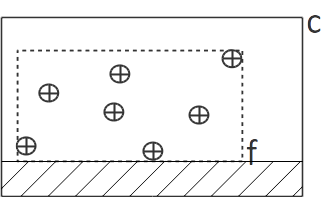
\includegraphics[width=0.8\textwidth]{figures/pac_rectangle}
    \subcaption{We want to guarantee that \\$P_{\dd}(\xx \in \mbox{bottom strip}) \leq \frac{\epsilon}{4}$.}
  \label{fig:pac_rect}
  \end{subfigure} \hfill%
  \begin{subfigure}[t]{0.48\textwidth}
    \centering
    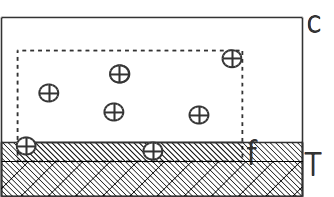
\includegraphics[width=0.8\textwidth]{figures/pac_rectangle_strip1}
    \subcaption{Favorable scenario: $T$ is larger than our bottom strip.}
    \label{fig:pac_rect_favorable}
  \end{subfigure}
  \begin{subfigure}[t]{0.48\textwidth}
    \centering
    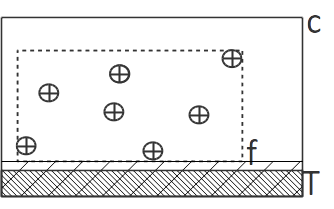
\includegraphics[width=0.8\textwidth]{figures/pac_rectangle_strip2}
    \subcaption{Scenario to avoid: $T$ is narrower than our bottom strip and we cannot guarantee that \\$P_{\dd}(\xx \in \mbox{bottom strip}) \leq \frac{\epsilon}{4}$.}
    \label{fig:pac_rect_bad}
  \end{subfigure} \hfill
  \begin{subfigure}[t]{0.48\textwidth}
    \centering
    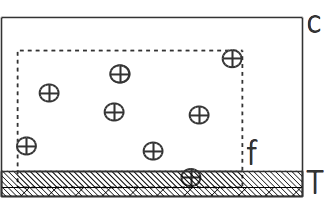
\includegraphics[width=0.8\textwidth]{figures/pac_rectangle_strip3}
    \subcaption{If a positive example was to fall in $T$, $f$, being the most specific hypothesis, would stretch to include it, and we would be in the favorable scenario.}
    \label{fig:pac_rect_bad_positive}
  \end{subfigure}
\caption{Learning an axis-aligned rectangle $c$. $f$ is the most specific hypothesis. Only the positive training examples are represented; the negative training examples all fall outside of $f$.}
\end{figure}

\section{Beyond binary classification}
\subsection{Multi-class classification}
Multi-class classification is the setting in which we want to learn $K>1$ classes $\cc_1, \dots, \cc_K$. Ffor example, instead of just learning ``family cars'', we now want to learn ``family cars'' but also ``luxury sedans'' and ``sports cars''.

The labels $\{\yy^i, \dots, \yy^K\}$ are now $k$-dimensional: $y_k^i = 1$ if and only if $\xx^i \in \cc_k$. Multi-class classification can be formulated as learning $k$ hypotheses $f_1, \dots, f_k$. This is often refered to as {\em one-vs-all classification}.

\subsection{Regression}
In regression, the labels are real-valued: $y^i \in \mathbb{R}$. 

The empirical error is given as:
\[
E(f|\dd) = \frac{1}{n}\sum_{i=1}^n (f(\xx^i) \neq y^i)^2.
\]


\end{document}




